\documentclass{article}                                                                                                                                   \usepackage{graphicx}
\usepackage[utf8]{inputenc}
\usepackage {enumitem}
\begin {document}
\begin{center}
\textbf {Arithematic Progression}
\end{center}                                                                                                                                              \begin {enumerate}
\item If the ratio of the sum of the first n terms of two A.Ps is $(7n+1):(4n+27)$, then find the ratio of their 9$^{th}$ terms.
\end {enumerate}                                                                                                                                                                                                                                                                                                    \begin{center}
\textbf{Trignometry}
\end{center}                                                                                                                                              \begin {enumerate}                                                                                                                                                                                                                                                                                                  \item From the top of the tower, $100$ m high, a man observes two cars on the opposite sides of the tower and in same straight line with its base, with angles of depression $30^{\circ}$ and $45^{\circ}$. Find the distance between the cars. [Take $\sqrt{3}$ = 1.732]

\end {enumerate}
\begin{center}
\textbf {Aptitude}                                                                                                                                        \end{center}
\begin {enumerate}
\item $A$ takes $6$ days less than $B$ to do a work. If both $A$ and $B$ working together can do it in $4$ days, how many days will $B$ take to finish it ?
        \end {enumerate}
 \begin{center}
\textbf{Probability}
\end{center}
\begin {enumerate}
                                                                                                                                                          \item Two different dice are thrown together. Find the probability that the numbers obtained have \begin{enumerate}[label=(\roman*)]                  \item even sum,and                            \item even product.                                   \end{enumerate}                                           \end {enumerate}
\begin{center}
\textbf{Algebra}
\end{center}                                                                                                                                              \begin{enumerate}                                                                                                                                         \item If the roots of the equation $(a^2 + b^2) x^2 - 2(ac+bd)x + (c^2 + d^2)=0$ are equal, prove that $\frac{a}{b} = \frac{c}{d}$.\\                     \item If the points $A(k+1,2k)$, $B(3k,2k+3)$ and $C(5k-1,5k)$ are collinear, then find value of $k$.                                                                                                                                                                                                               \item Solve for $x$:\\                                                                                                                                                                    $\frac{x-1}{2x+1} + \frac{2x+1}{x-1} = 2$,
                where $x \neq - \frac{1}{2},1$                                                                                                                            \end{enumerate}
                                                                                                                                                                                                                                                                                                                    \begin {center}                               \textbf{Geometry}
\end {center}                                                                            \begin{enumerate}                                      \item Construct a triangle $ABC$ with side $BC$ = $7$ cm, \angle $B$ = $45^{\circ}$ , \angle $A$ = $105^{\circ}$. Then construct another triangle whose sides are $\frac{3}{4}$ times the corresponding sides of the $\Delta$ ABC.                                  \item In a rain-water harvesting system, the rain-water from a roof of $22$ m x $20$ m drains into a cylindrical tank having diameter of base $2$ m and height $3.5$ m. If the tank is full, find the rainfall in cm. Write your views on water conservation.                       \item Prove that the lengths of two tangents drawn from an external point to a circle are equal.                                          \item In the given figure, $XY$ and $X'Y'$ are two parallel tangents to a circle with center $O$, and another tangent $AB$ with point of contact $C$ is intersecting $XY$ at $A$ and $X'Y'$ at $B$. Prove that \(\angle AOB = 90^\circ\).
 \begin{figure}[h!]                             \centering                                    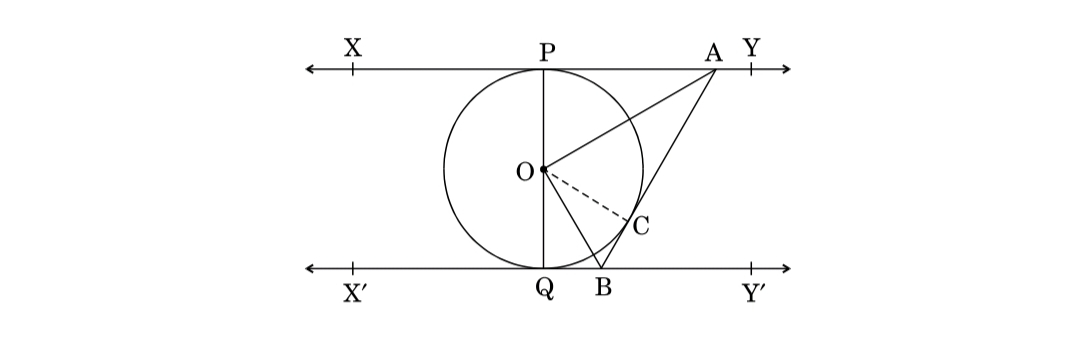
\includegraphics[width=0.8\textwidth]{figjpg.jpg}                             \caption{fig.jpg}                             \label{fig:fig.jpg}           \end{figure}
 \item In the given figure, $O$ is the centre of the circle with $AC$ = $24$ cm, $AB$ = $7$ cm and \angle $BOD$ = $90^{\circ}$. Find the area of the shaded region.                              \begin{figure}[h!]                                \centering                                    
\includegraphics[width=0.8\textwidth]{figjpg (1).jpg}

                \caption{fig.jpg}                             \label{fig:fig.jpg}                   \end{figure}
 \end{enumerate}
\end {document}
